\section{Chapter Overview}

This chapter covers the methodology used in our project. It covers in detail the different steps that we took in the entire project. As discussed by Rachiele, methodology in software development is a process that includes a number of tasks by default being; planning, creating, testing and finally deployment \cite{SDM}. Besides this, methodology in software development is professionally based on a prescribed process which develops use to be timely, organised and structured.  
\newline
\newline
There is a number of methodologies that are suitable for this project. This includes but is not limited to Agile, Scrum and the Waterfall method. After careful consideration we agreed to use the Waterfall method for project management. 
\newline
\newline
The Waterfall method was picked because of its applicability to develop a POS system where every phase is intertwined and rely on other completion of singular phase sequentially for resources to be released for the next phase. For example the products table could not be started unless the categories table was complete as it needs a category to be saved to the database. The project is full of scenarios similar to this rendering the Waterfall method as the most viable option.


\section{Meeting}

Meetings between team members took place every week. Initially we had meetings twice a week to develop quorum as well as a rudimentary plan which would then be adopted as the project methodology. We then settled for once a week meeting which was sufficient as we developed the work remotely. [fig].

%\begin{figure}[h!]
%	\caption{Meeting.}
%	\label{image:myImageName}
%	\centering
%	
\includegraphics[width=0.9\textwidth]{Fig images/notsure.jpg}
%\end{figure}

The meeting would start with discussing the things we have learned since the last meeting. This part of the meeting was vital as we had to be on the same level when learning a new language. Very early on in the project we identified several online tutorials where we could learn the fundamentals of the PHP programming language \cite{W3}. At the end of every meeting we would set a couple of milestones we would have to have achieve development wise before the next time meeting. These meeting usually corresponded with certain parts of the language we needed to learn in order to complete the project. 






\section{Problem Solving}

From the inception of the project we knew that learning a new language was going to cause a number of minor problems throughout the project. We therefore devised a problem solving process which would guide us and therefore we adhered to it throughout the development life-cycle. We therefore ensured that the learning curve was manageable and pointed towards the success of the project. We further established boundaries as far as our learning and problem solving capabilities are concerned to ensure we remained on course as we made relevant research and consultations. 
\newline
\newline
Problems were solved by scheduling a meeting and discussing the problem at hand. The problem was then broken down into small steps where each team member was designated a task to research and solve. Another meeting would then take place to put the code together and test it to see if it worked. This approach really benefited us as we both learned a lot about the parts of the project in which we weren't directly involved. Working as a teams also ensured that we complemented and supplemented each other where necessary. The process also ensured we developed a continued learning culture while we furthered aid in developing updates and more ground breaking technologies. 
\newline
\newline
Part of the critical steps in problem solving is constantly consulting with the market players to ensure that we solve existing challenges. This was done after our research work indicated  that often developers work resolved around assumed or inaccurate challenges. This is a result of poor problem solving skills. We therefore maintained regular consultations with our potential clients to ensure each and every build was oriented to solving their problems. 


\section{Version Control}

GitHub

In order to work on the project as a team while maintaining industrial standards, we required a number of tools to control and manage our work. After researching on potential collaboration tools we agreed to use GitHub and Microsoft Teams. GitHub offered us various tools to aid in the planning, tracking and development of our project. Throughout our project we used GitHub as our version control tool. 
\newline
\newline
One specific areas where GitHub was quite collaborative is the creation of the repository and adding the members of the team to work as collaborators the GitHub’s task management tool. This ensured that both team members had valid contribution to the project. Further it enabled us to supplement our skills where necessary. Using GitHub also enabled us to consult on very specific areas of coding strictly on system engineering and system design. This ensured that the project maintained professional control framework as far as industry standard is concern.  
\newline
\newline
We then proceeded to building our Kanban board, posting every task to it in order to keep track of where we were and what was expected next. This allowed us to break down our tasks into smaller, more manageable tasks. Through the utilization of its features we found GitHub to be an extremely useful tool in the research and development of our project as it allowed us to keep track of code, tasks and errors all in the one place. The Kanban board also assisted in the documentation of the project avoiding instances where different documentation structures and process would be required. This provides grounds for further research as well as future updates to the program by reviewing the challenges and steps taken to resolve them. 
\newline
\newline
Use of GitHub also enabled us to be responsible developers in the information communication industry. By documenting our work in the platform, we provide grounds for other developers to research on similar projects. This meant that we were open to “public” scrutiny and opinion by contributing in a productive and illustrative manner. Overall GitHub plays a vital role in bring developers on-board and we were proud of contributing to the efforts. 
Using Microsoft Teams allowed us to keep in contact with each other and our project supervisor via messaging and video chats. Utilizing its share screen function we were able to both have an input into sections of the projects being covered by the other person. This was especially beneficial after the outbreak of the covid-19 virus which restricted us from having face-to-face meetings.


\section{Selection Criteria}

After laying out the problem statement, project proposal and problem objectives we finally had to start the actual build. We therefore embarked on a selection process, where we derived the best languages and additional tools that would be best for the project. This meant that we had to self-evaluate and reflect on the goals of the project. This stage was easily determined a vital step in the project milestones.
The selection criteria for our project and indeed any project is key and something that must be laid out clearly. When selecting our languages, platforms and technologies we needed to ensure that all platforms would meet a certain standard that would enable us to tackle the challenges that were foreseeable in the different stages from beginning to completion.
\newline
\newline
We had to make sure that the language chosen was not only a language worth learning but also one that would be able to help us build the project as efficiently as possible. The technologies chosen had to be capable of running what we were building and be compatible with future hardware and software developments.


 
\section{Development Methodology}

\subsection{Waterfall}

According to tutorial points editorials, the waterfall model is a simple to use approach where one phase must be completed before the next phase begins while avoiding overlapping \cite{WFM}. The tutorial points outlines the bases of the model as a linear sequential flow. The Waterfall model requires the following of sequential phases throughout the software development cycle, starting with initial instructions regarding a customer’s specific requirements followed by the practical implementation and product construction. Using the waterfall method leaves little room for change as the project proceeds therefore initial planning has to be thorough and every aspect of the project has to be designed and addressed before we could move on to the next stage.

\begin{figure}[h!]
	\caption{Waterfall Methodology.}
	\label{image:myImageName}
	\centering
	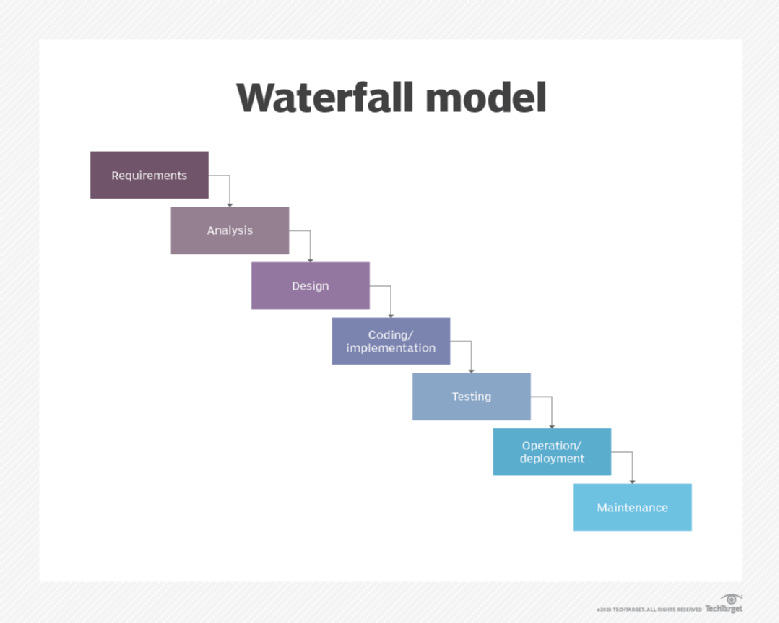
\includegraphics[width=0.9\textwidth]{Fig images/waterfall.png}
\end{figure}

The following are the steps involved in the Waterfall process and how we incorporated them into the building of our project. We will give a brief summary of the process as well as explaining which meetings we held to discuss which step. 

\section{Conception}

This phase begins with the innovative idea we wish to develop. It involves a broad assessment of the project, whether or not it is viable and why it is beneficial to the individual team members.
To begin with, we decided to have meetings twice a week to discuss the ideas for the project and what we would be interested and productive to work on. In these initial meetings, we discussed the various projects we could undertake and whether or not they would be worthy of a 15 credit, level 8 module. 
\newline
\newline
A POS system was the first project that we proposed because of its complexity. The project was also viable because of the number years we spent working in areas using a till system, something we both had a strong understanding of, and knew the work around different systems and how to improve them. 
\newline
\newline
We also looked at other ideas such as websites and applications that could buy and sell products among other things. These were all good ideas but we knew that, with our deep understanding and experience with POS systems, we could make a change and develop better systems that solve client problems. We didn’t just want our project to be good, we wanted it to stand out and be worthy of a higher grade.
\newline
\newline
The next step in the process was the language. Learning a new language was always something that we put a lot of consideration in to as we knew learning something new would benefit us. In a lecture by Dr. John Healy he mentioned that we all should look at the possibility of learning a new language in order to broaden our knowledge in a chosen field. We therefore made a decision to explore the learning curve of a new programming language.
\newline
\newline
After a vast research into which programming languages we could use, PHP came up time and time again, as a great solution to what we were trying to achieve. Given that PHP is an Object-Oriented language we thought it ticked all the boxes that we needed to achieve our goal of building our POS system. 

\section{Initiation} 

Once the idea is agreed upon we began to define objectives, scope, purpose and deliverables of the project. At this stage we put together a list of the different steps we needed to take to complete every step of the project and move on to the next phase. In this stage we made sure the potential clients for the system had made their submissions as far as a viable POS and RMS are concerned.
After combining our joint experience of POS systems we put together a list of features the system must have to be considered viable and suitable for use. The list is found above under the objectives heading.

\section{Requirement Gathering and Analysis}

This part of the process required team members to research and identify all possible requirements of the POS system we aimed to develop. Specific functionality of each component must be identified, addressed and carefully thought out and documented before moving on to the next phase of production.
\newline
\newline
This process took time, with several meetings conducted to address different ways in which we would approach the build process. This was complimented using our own knowledge and experience of POS systems we researched extensively into what makes a good POS system and what parts of existing systems are better left out. This was a critical step in ensuring we develop a system that address challenges in the field as opposed to developing systems that solve developer quest for flashing software. We therefore made sure we incorporate the different actors’ opinion on the issue in rational and professional manner.

\section{System Design}

In this phase the system specifications from the previous phase are addressed, and the system design is discussed and agreed upon. The system design helps specify the overall system architecture of the project whilst also specifying hardware and system requirements needed to complete this project.  In this phase we reviewed the complex requirements of a POS amalgamated with a RMS ensuring that all the characteristics are built into the systems. In the System Design chapter we will take a more in depth look at this process and how we approached it.

\section{Implementation}

Using inputs from the system design, the system is differentiated into smaller units. This smaller units are then build based on the systems design and system objectives. This phase carries the most regal room as far problem solving is concerned. We therefore made sure we paid attention to detail, constantly consulted and made sure development remained on course. We then integrated the units into the next phase of the project cycle. Each unit is developed and tested to ensure it is the best fit for the intended purpose and that its functionality runs as it is intended to run. 

\section{Integration and Testing}

When all units are developed and tested, they are integrated into the main system. Post-integration, the entire system is fully tested to ensure that there are no faults. In this process we used Microsoft Teams to ensure both of us observed the results of these tests. We will delve more into the testing process in the testing chapter later in this paper.

\section{Deployment of system}
??????????
When the system was built and fully functional and all the testing was done the product was deployed onto the CLOUD???? Again we used Microsoft Teams to view this process as it happened.

\section{Chapter Summary} 


%References

%[1] 	G. Rachiele, "Software Development Methodologies," Medium, 9 April 2018. [Online]. Available: https://medium.com/@gianpaul.r/software-development-methodologies-a856883a7630. [Accessed 12 April 2020].
%[2] 	w3schools, "PHP Tutorial," w3schools, 2020. [Online]. Available: https://www.w3schools.com/PHP/DEfaULT.asP. [Accessed 12 April 2020].
%[3] 	Tutorial Points, "SDLC - Waterfall Model," Tutorial Points, 2020. [Online]. Available: https://www.tutorialspoint.com/sdlc/sdlc_waterfall_model.htm. [Accessed 12 April 2020].










